\documentclass{article}

\usepackage[a4paper, total={6.5in, 9in}]{geometry}
\usepackage{tikz}
\usepackage{gensymb}
\usepackage{float}
\usetikzlibrary{shapes.geometric, arrows}

% Chart Setup
\tikzstyle{boxes} = [rectangle, minimum width=2cm, minimum height=1cm, text centered, text
width=2cm, draw=black]

\tikzstyle{bar} = [rectangle, minimum width=15cm, minimum height=1cm, text centered, text
width=15cm, draw=black]

\tikzstyle{intNode} = [diamond, minimum width=2cm, minimum height=1cm, text centered, text
width=2cm, draw=black]

\tikzstyle{arrow} = [thick, ->, >=stealth]

\title{Kelvin Barnsdale Guest Lecture Summary}
\author{Josiah Craw\\35046080}

\begin{document}

\maketitle

This guest lecture was presented by Kelvin Barnsdale from RF Engineering services Ltd. Firstly
Kelvin discussed the prerequisites for a successful development program. These things are:

\begin{enumerate}
    
    \item{Passion for the product}

    \item{Market intelligence}

    \item{Product requirements}

    \item{Having the necessary tools and resources}

\end{enumerate}

Kelvin next covered the two major development methods, waterfall and agile. Kelvin talked about
the advantages and disadvantages of each, for waterfall the main points of it are:

\begin{itemize}

    \item{product requirements and specifications are agreed upon up front}

    \item{The progress is measured}

    \item{Team members do not need to be dedicated to one part of the project}

\end{itemize}

The key part of agile are as follows:

\begin{itemize}

    \item{Fast}

    \item{Lots of customer interactions}

    \item{The customer assumes some ownership}

    \item{Iterations can be market tested}

    \item{Changes in the specifications can be made part way into the project}

\end{itemize}

\begin{figure}[H]
\centering
\begin{tikzpicture}

    \node (start) [boxes] {Start};

    \node (req) [boxes, below of=start, right of=start, xshift=2cm] {Requirements};

    \node (des) [boxes, below of=req, right of=req, xshift=2cm] {Design};

    \node (imp) [boxes, below of=des, right of=des, xshift=2cm] {Implement};

    \node (ver) [boxes, below of=imp, right of=imp, xshift=2cm] {Verify};

    \node (del) [boxes, below of=ver, right of=ver, xshift=2cm] {Deliver};

    \draw[arrow] (start) -| (req);
    \draw[arrow] (req) -| (des);
    \draw[arrow] (des) -| (imp);
    \draw[arrow] (imp) -| (ver);
    \draw[arrow] (ver) -| (del);

\end{tikzpicture}
\caption{Demonstration of the waterfall development process}
\end{figure}

\begin{figure}[H]
\centering
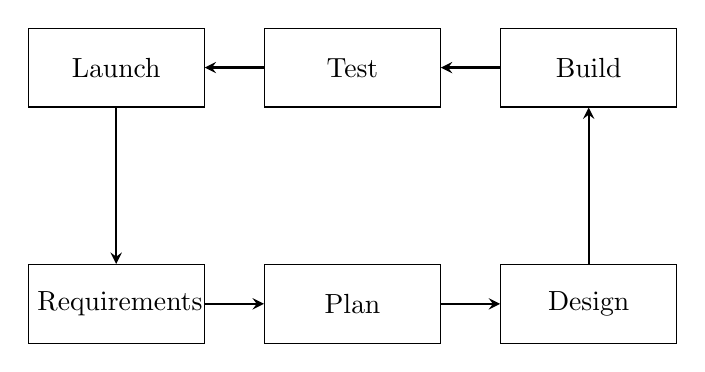
\begin{tikzpicture}

    \node (start) [boxes] {Requirements};

    \node (plan) [boxes, right of=start, xshift=2cm] {Plan};

    \node (des) [boxes, right of=plan, xshift=2cm] {Design};

    \node (build) [boxes, above of=des, yshift=2cm] {Build};

    \node (test) [boxes, left of=build, xshift=-2cm] {Test};

    \node (launch) [boxes, left of=test, xshift=-2cm] {Launch};

    \draw[arrow] (start) -- (plan);
    \draw[arrow] (plan) -- (des);
    \draw[arrow] (des) -- (build);
    \draw[arrow] (build) -- (test);
    \draw[arrow] (test) -- (launch);
    \draw[arrow] (launch) -- (start);

\end{tikzpicture}
\caption{Demonstration of the Agile development process}
\end{figure}

The next part of a successful development program is the product requirements specifications
(PRS). This document contains all of the specifications for a design. This document should be
written from a high level perspective and should describe the product as the customer/market
pictures it. This document should not contain specific details eg. an M5 bolt is to be used to
connect the PCB to the housing.

Kelvin next discussed the stage and gate process for PCB design, this is shown in
Figure~\ref{fig:stageAndGatePro}.

\begin{figure}[H]
\centering
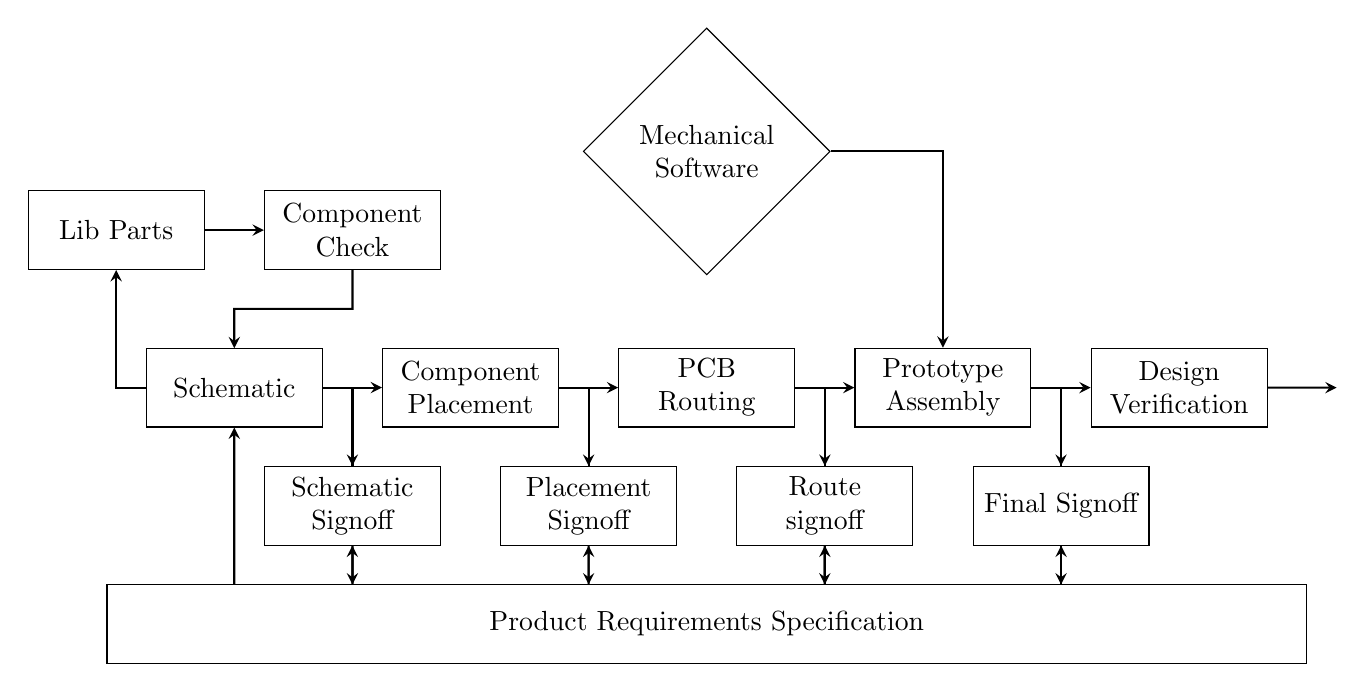
\begin{tikzpicture}

    \node (proBox) [bar] {Product Requirements Specification};

    \node (schem) [boxes, above of=proBox, yshift=2cm, xshift=-6cm] {Schematic};
    \node (libPart) [boxes, above of=schem, yshift=1cm, xshift=-1.5cm] {Lib Parts};
    \node (comCheck) [boxes, above of=schem, yshift=1cm, xshift=1.5cm] {Component Check}; 
    
    \node (comPlace) [boxes, right of=schem, xshift=2cm] {Component Placement};

    \node (route) [boxes, right of=comPlace, xshift=2cm] {PCB Routing};

    \node (assem) [boxes, right of=route, xshift=2cm] {Prototype Assembly};
    \node (input) [intNode, above of=assem, yshift=2cm, xshift=-3cm] {Mechanical\\Software};

    \node (desVer) [boxes, right of=assem, xshift=2cm] {Design Verification};

    \node (schemSign) [boxes, below of=schem, yshift=-0.5cm, xshift=1.5cm] {Schematic Signoff};
    \node (placeSign) [boxes, right of=schemSign, xshift=2cm] {Placement Signoff};
    \node (routeSign) [boxes, right of=placeSign, xshift=2cm] {Route signoff};
    \node (finalSign) [boxes, right of=routeSign, xshift=2cm] {Final Signoff};

    \draw[arrow] (-6, 0.5) -- (schem);
    \draw[arrow] (schem) -| (libPart);
    \draw[arrow] (libPart) -- (comCheck);
    \draw[arrow] (comCheck) -- (-4.5, 4) -| (-6, 3.5);
    \draw[arrow] (schem) -| (schemSign);

    \draw[arrow] (-4.5, 0.5) -- (schemSign);
    \draw[arrow] (schemSign) -- (-4.5, 0.5);

    \draw[arrow] (schemSign) |- (comPlace);

    \draw[arrow] (comPlace) -| (placeSign);
    \draw[arrow] (placeSign) |- (route);
    \draw[arrow] (placeSign) -- (-1.5, 0.5);
    \draw[arrow] (-1.5, 0.5) -- (placeSign);

    \draw[arrow] (route) -| (routeSign);
    \draw[arrow] (routeSign) |- (assem);
    \draw[arrow] (routeSign) -- (1.5, 0.5);
    \draw[arrow] (1.5, 0.5) -- (routeSign);

    \draw[arrow] (assem) -| (finalSign);
    \draw[arrow] (finalSign) |- (desVer);
    \draw[arrow] (4.5, 0.5) -- (finalSign);
    \draw[arrow] (finalSign) -- (4.5, 0.5);

    \draw[arrow] (input) -| (assem);

    \draw[arrow] (desVer) -- (8, 3);

\end{tikzpicture}
\caption{The stage and gate process for PCB design}
\label{fig:stageAndGatePro}
\end{figure}

The first sign off is the schematic sign off, this is the largest check with 52 points. This only
checks the design against product requirements specification. This process can avert issues in the
procurement, software, production, and manufacturing issues. The next check is the PCB component 
check this check checks the physical properties of the PCB and layout and makes sure the
components are placed correctly before routing. This check should be completed using a buddy
system should be done by a buddy, and it should be ensured that the foot print and schematics are
signed of together. Finally, the design verification test stage, for this stage a design
verification plan is made. This plan contains the items that are to be tested, these items are
pulled from the PRS. The best method for testing is to make testing features build into the design
of the product. The requirements for the product to pass the test should be contained within the
PRS.

Finally the take home points from this lecture are:
\begin{itemize}

    \item{Research the best design process eg. Agile or Waterfall}

    \item{Make sure you are conforming to specifications throughout the process}

    \item{Ensure reviews are made by others in the team at every stage}

    \item{Time spent at the beginning of the project ensuring the specifications are correct is
        worthwhile time spent}

\end{itemize}

\end{document}
